\section{Supplementary Figures}\label{sec:SupplementaryFigures} 


\begin{figure}[h]
    \centering
    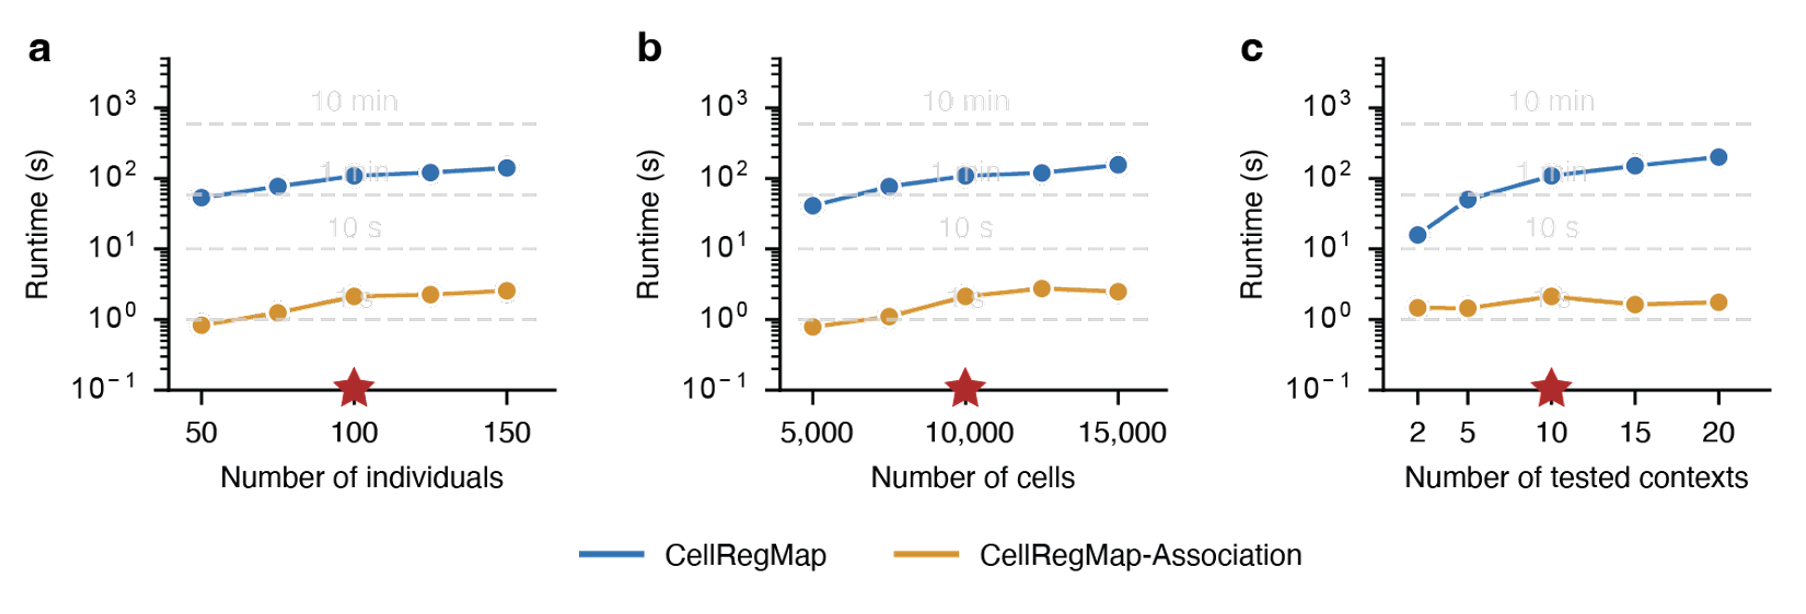
\includegraphics[width=16cm]{Appendix_CellRegMap/SuppFigures/Fig_S1.png}
    \caption{\textbf{Empirical assessment of the computational complexity of CellRegMap and CellRegMap-Association test.} 
    Shown are empirical runtimes for simulated data (setup as described in \textbf{Materials and Methods}) averaged across 150 eQTL. 
    Runtimes evaluated on an Intel Xeon CPU E5-2660 v4 with 2.00GHz. 
    Shown are runtimes (y-axis) for testing a single eQTL as a function of the number of individuals \textbf{(a)}, the total number of cells \textbf{(b)} and the number of context variables \textbf{(c)}; runtimes are evaluated for both the CellRegMap model (interaction test, blue), and the corresponding association test (orange). 
    Stars highlight default values for fixed parameters. 
    All parameters retained at their default parameter values except the parameter that is indicated on the x axis.}
\end{figure}

\begin{figure}[htb!]
    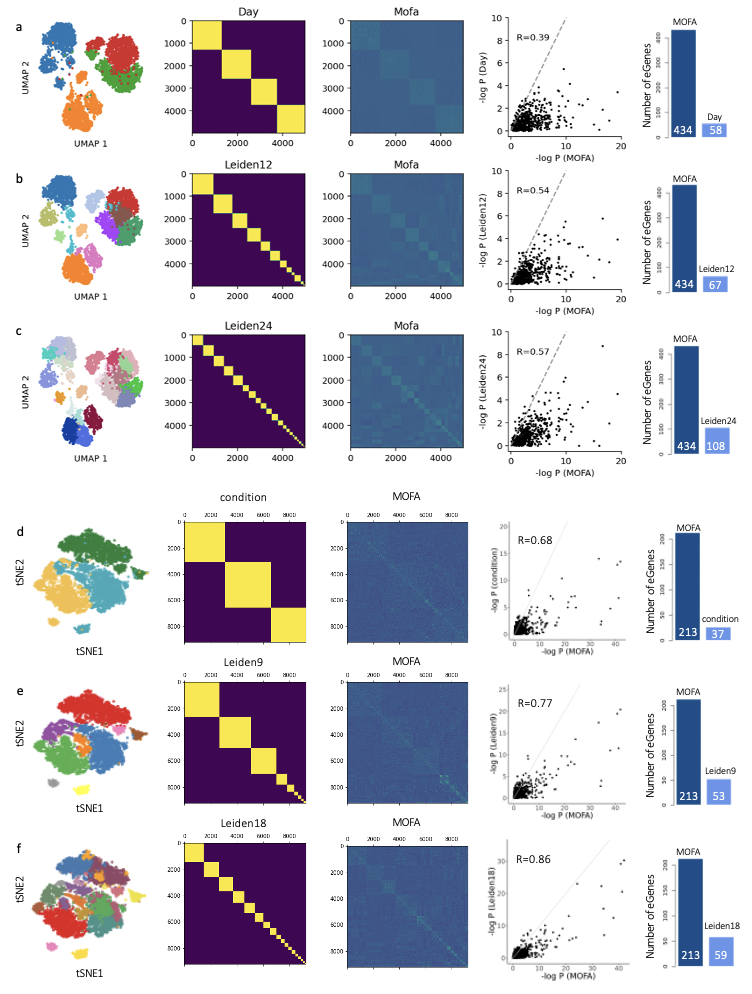
\includegraphics[width=15cm]{Appendix_CellRegMap/SuppFigures/Fig_S2.png}
    \caption{\textbf{Comparison of CellRegMap when using discrete cell contexts instead of continuous cell contexts on simulated and real data (Full legend on next page).}\\}
    \label{suppl_fig:immunostaining}
\end{figure}

\clearpage


\small{\textbf{Comparison of CellRegMap when using discrete cell contexts instead of continuous cell contexts on simulated and real data (continued).}
Concordance of results when using discrete vs. continuous contexts for CellRegMap. 
\textbf{Left:} 2-dimensional visualisation of the gene expression data and discrete clusters. 
\textbf{Middle:} Discrete and continuous covariance matrices (based on MOFA factors) sorted by cluster membership. 
\textbf{Right:} Result comparison; -log10(P-values) comparing models using continuous (x-axis) vs discrete (y-axis) contexts, as well as bar plots showing the number of significant GxC eQTL identified using the different context-covariance matrices.
(a-c) Results for 500 semi-synthetic eQTL as used for the results presented in main text \textbf{Fig. 2} for the setting of 10 leading MOFA factors and the fraction of genetic variance explained by GxC = 0.5 (\textbf{Materials and Methods}).
We consider discrete contexts at three different resolutions: \textbf{(a)} the original 4 sampling time points (Day), \textbf{(b)} 12 and \textbf{(c)} 24 Leiden clusters. 
Number of significant eGenes is out of 500 tested (FDR $<$ 10\%). 
(d-f) Results on real data, considering the neuronal differentiation data from \cite{jerber2021population}. 
Results from running CellRegMap with 8,479 pseudo cells (\textbf{Materials and Methods}) and testing 2,051 eQTL (1,374 eGenes) in dopaminergic neurons from the original study. 
We compare results when using, as contexts, \textbf{(d)} the three discrete conditions from the original study (day 30, day 52 and rotenone-treated day 52; “condition”), \textbf{(e)} 9 and \textbf{(f)} 18 Leiden clusters, as opposed to 10 continuous MOFA factors, as done in the main analysis. 
Number of significant eGenes is out of 1,374 tested (FDR $<$ 5\%, to match results from the main analysis).} 

\begin{figure}[h]
    \centering
    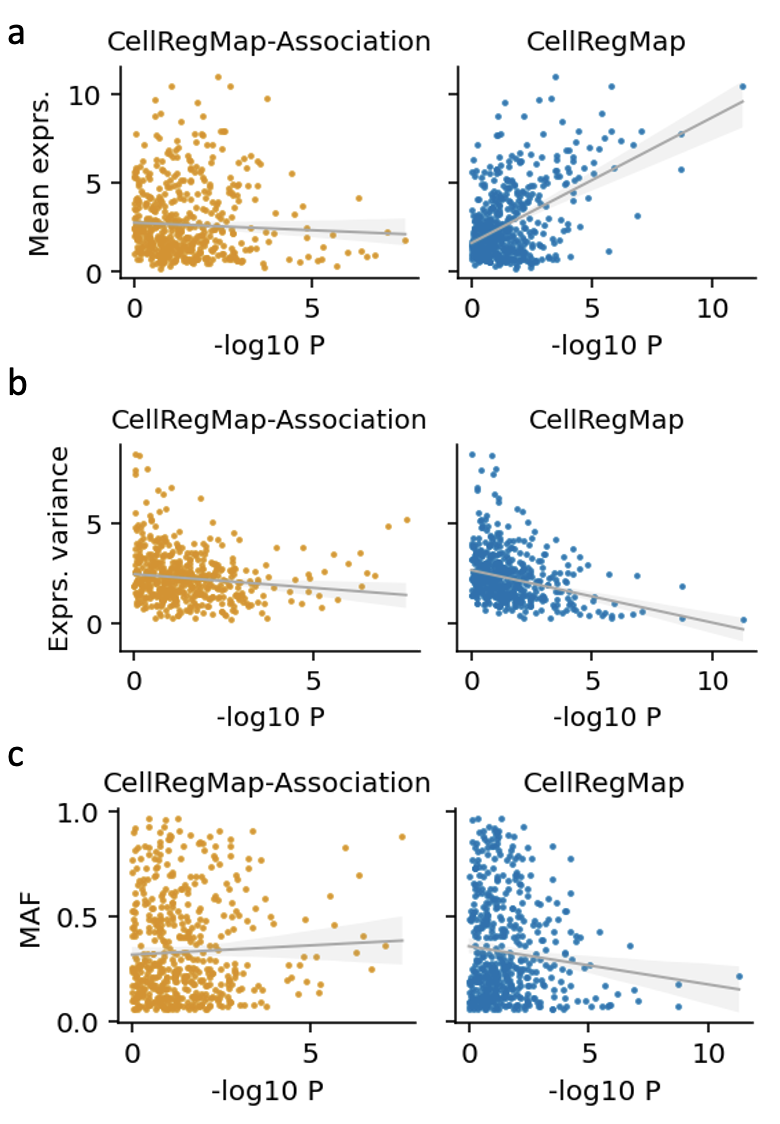
\includegraphics[width=10cm]{Appendix_CellRegMap/SuppFigures/Fig_S3.png}
    \caption{\textbf{eQTL statistics stratified for gene properties on simulated data.}
    Results for simulated genetic effects using the same parameters as in \textbf{Appendix Fig. S2} (10 MOFA factors with GxC, fraction of genetic variance explained by GxC = 0.5; \textbf{Materials and Methods}). 
    Shown are the \textbf{(a)} mean observed gene expression of the simulated eGene (prior to adding the genetic effect), \textbf{(b)} the prior gene expression variance and \textbf{(c)} the minor allele frequency as a function of the P-value estimated by CellRegMap (blue) and CellRegMap-Association (orange). 
    Both models are fitted using the same set of ground truth context variables as used in the simulation. 
    Lines show the regression fit and shaded areas 95\% confidence intervals.
}
\end{figure}

\begin{figure}[h]
    \centering
    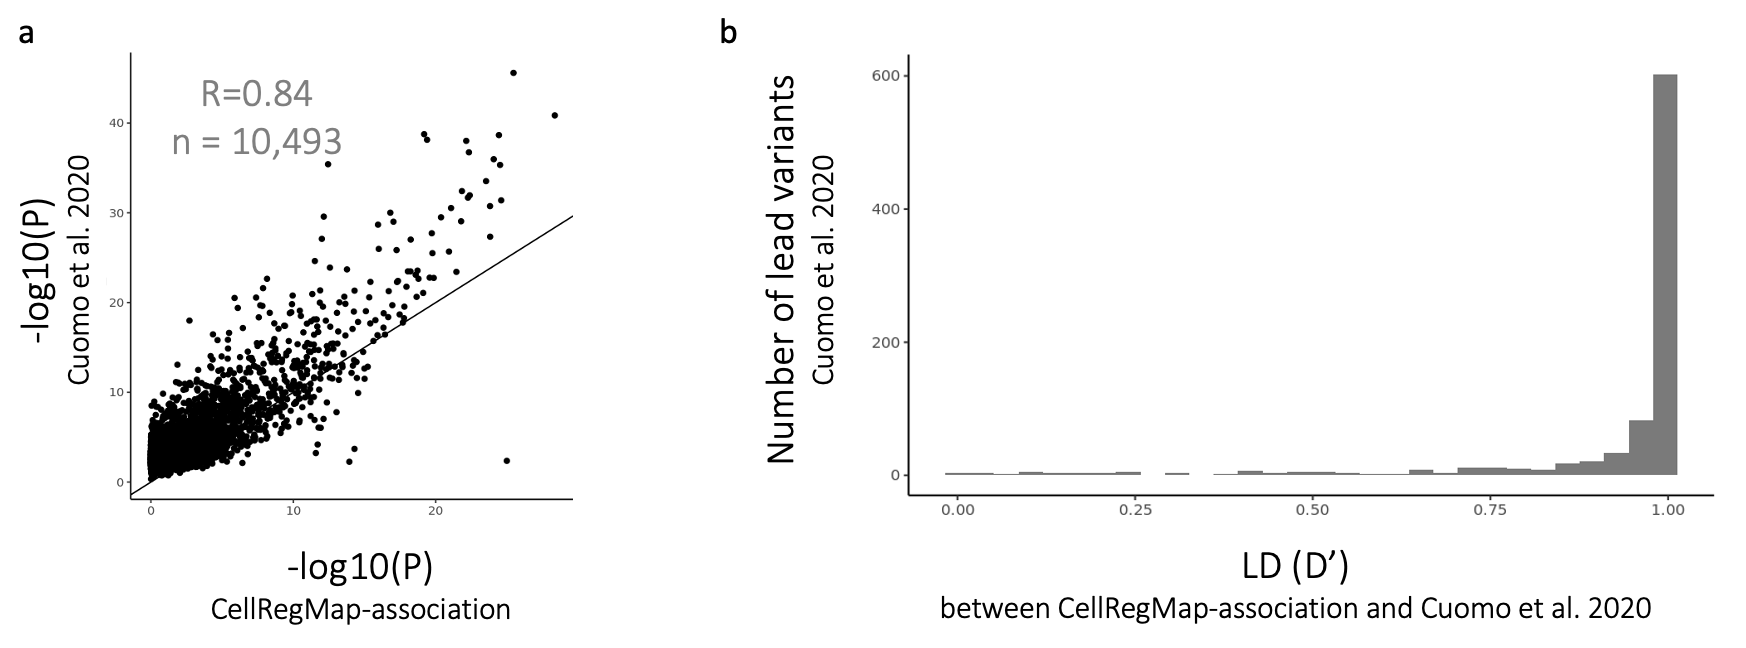
\includegraphics[width=16cm]{Appendix_CellRegMap/SuppFigures/Fig_S4.png}
    \caption{\textbf{Concordance of persistent genetic effects on endoderm differentiation data.}
    Data from \cite{cuomo2020single}. 
    \textbf{(a)} Scatter plot of -log10 p-values from the original study (\cite{cuomo2020single}, y-axis) vs -log10 p-values when using the CellRegMap-association test (x-axis). 
    For the published study, the top variant from each gene is considered (n=10,493 genes). 
    These results were achieved using aggregated “pseudocounts” from each of the three stages, and for each gene-SNP pair we are here selecting the smallest p-values between the iPSC, mesendoderm and definitive endoderm eQTL. 
    \textbf{(b)} For each of the significant eGenes from the original study (n=2,996), we assessed whether the lead variant identified was the same or in linkage disequilibrium (LD) with the lead variant identified by CellRegMap-association. 
    Histogram of the LD (D’, as calculated using the R package “LDlinkR”, \cite{myers2020ldlinkr}) distribution between lead variants from the two tests.
}
\end{figure}

\begin{figure}[h]
    \centering
    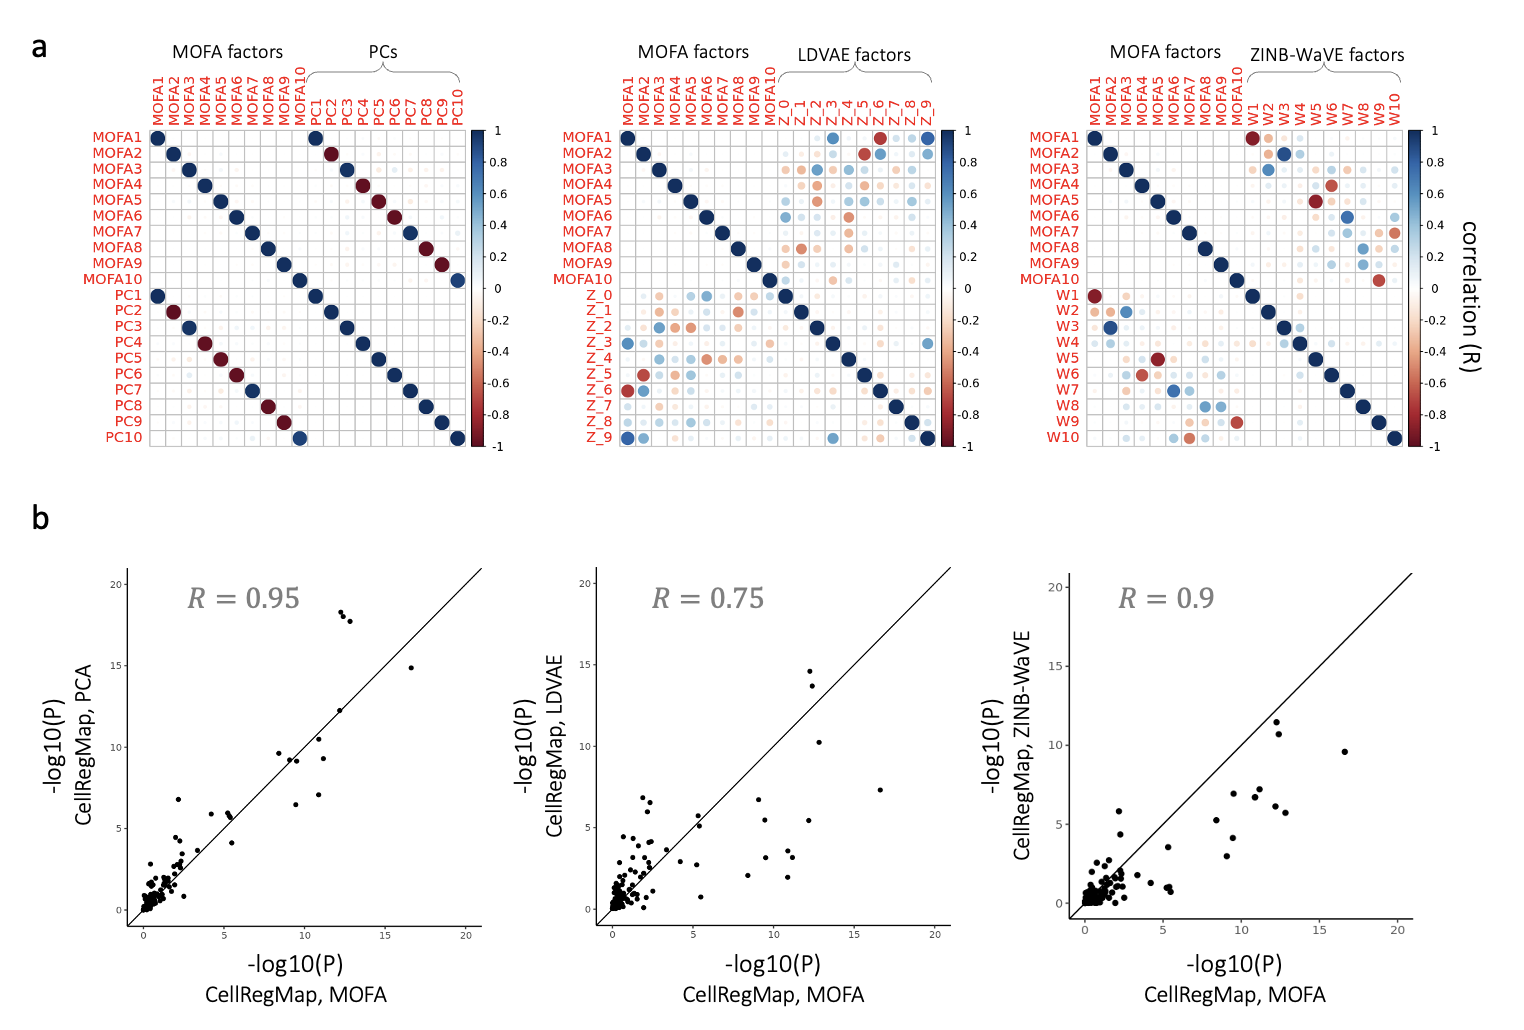
\includegraphics[width=16cm]{Appendix_CellRegMap/SuppFigures/Fig_S5.png}
    \caption{\textbf{Comparison of alternative methods to define cellular contexts.}
    Assessment based on the endoderm differentiation study \cite{cuomo2020single}. 
    We compared the MOFA workflow to define cellular contexts to principal component analysis (left), linearly-decoded variational autoencoder (LDVAE \cite{svensson2020interpretable}, middle) and zero-inflated negative binomial-based wanted variation extraction (ZINB-WaVe \cite{risso2018general}, right). 
    \textbf{(a)} Correlation matrix between the leading 10 factors identified by MOFA and the respective alternative method.  
    \textbf{(b)} Scatter plot of negative log p-value of the CellRegMap interaction test when using MOFA cell contexts (x-axis) versus using a cell-context covariance derived using the respective alternative method (y-axis). 
    Considered are n=121 SNP-gene pairs from 88 unique genes on chromosome 22 only.
}
\end{figure}

\begin{figure}[h]
    \centering
    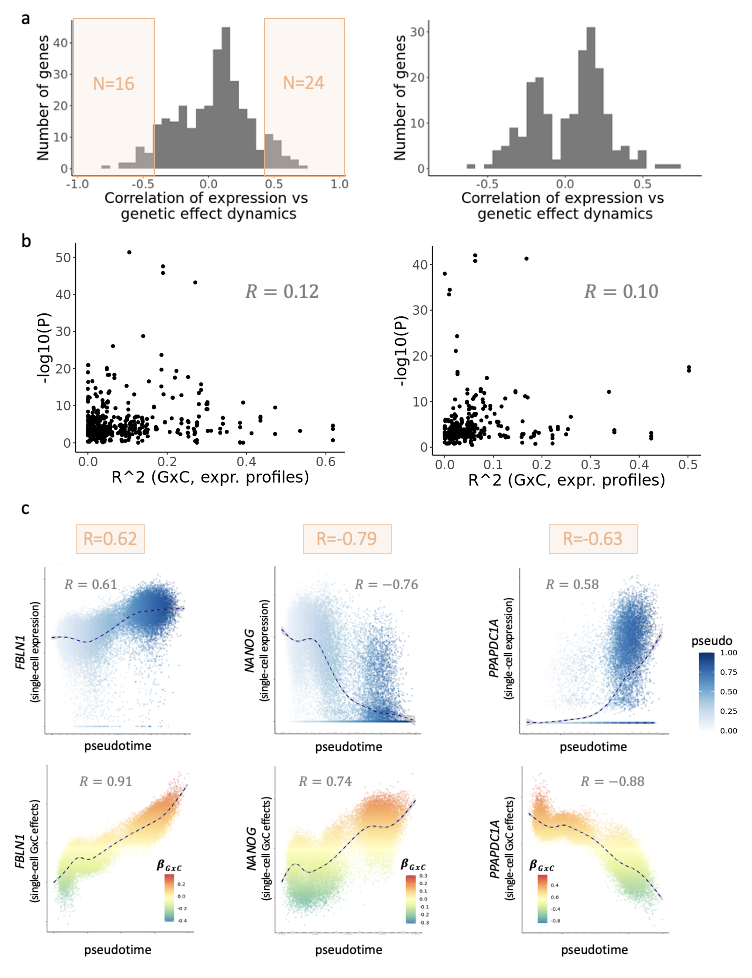
\includegraphics[width=11cm]{Appendix_CellRegMap/SuppFigures/Fig_S6.png}
    \caption{\textbf{Correlations of GxC with gene expression dynamics.}
    \textbf{(a)} Correlation (R) between single-cell expression profiles and estimated single-cell genetic effect profiles for 322 and 213 genes with significant GxC effects respectively (FDR$<$5\%) (left: endoderm differentiation data from Cuomo et al \cite{cuomo2020single}, right: neuronal differentiation data from Jerber et al \cite{jerber2021population}). 
    \textbf{(b)} Scatter plot between the R2 correlation coefficient between gene expression and GxC (x axis, as in \textbf{a}, but considering R2 instead of R) versus the statistical significance of GxC effects (-log10(p-value), y axis)  (left: endoderm differentiation data from Cuomo et al, right: neuronal differentiation data from Jerber et al). 
    \textbf{(c)} For three examples from a (high $|$R$|$ between expression and GxC effects dynamics), the top row represents single-cell expression the genes (y-axis) as a function of pseudotime (x-axis); the bottom row represents the single-cell genetic effect estimates due to GxC (y-axis) as a function of pseudotime (x-axis). 
    In orange, the R coefficient between expression and GxC effect dynamics, as in \textbf{a}.
}
\end{figure}

\begin{figure}[h]
    \centering
    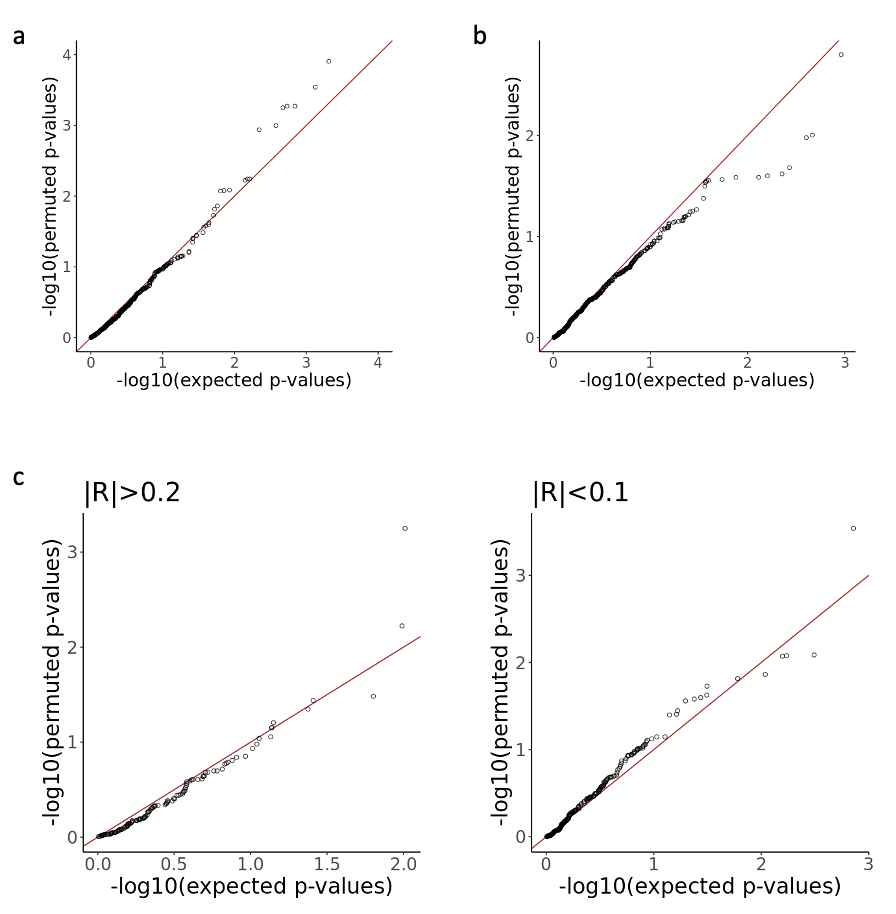
\includegraphics[width=13cm]{Appendix_CellRegMap/SuppFigures/Fig_S7.png}
    \caption{\textbf{Calibration of CellRegMap in relation to expression dynamics.}
    Shown are results obtained from the endoderm differentiation data \cite{cuomo2020single}; (GxC interaction test) considering genes on chromosome 22 only. 
    QQplots demonstrating calibration using permitted genotypes (GxC component only) \textbf{(a)} Across all gene-SNP pairs from (n=540, i.e. 270 genes, 2 SNPs each): median=0.57. 
    \textbf{(b)} Across all gene-SNP pairs from (neuron differentiation data from Jerber et al, [3]) (n=500, i.e. 250 genes, 2 SNPs each): median=0.51. 
    \textbf{(c)} Considering the endoderm differentiation data, as in a, but stratifying genes by those whose expression is (left) correlated with differentiation time ($|$R$|>$0.2; n=134, median=0.51) and (right) not correlated with differentiation time ($|$R$|<$0.1; n=218, median=0.47).
}
\end{figure}

\begin{figure}[h]
    \centering
    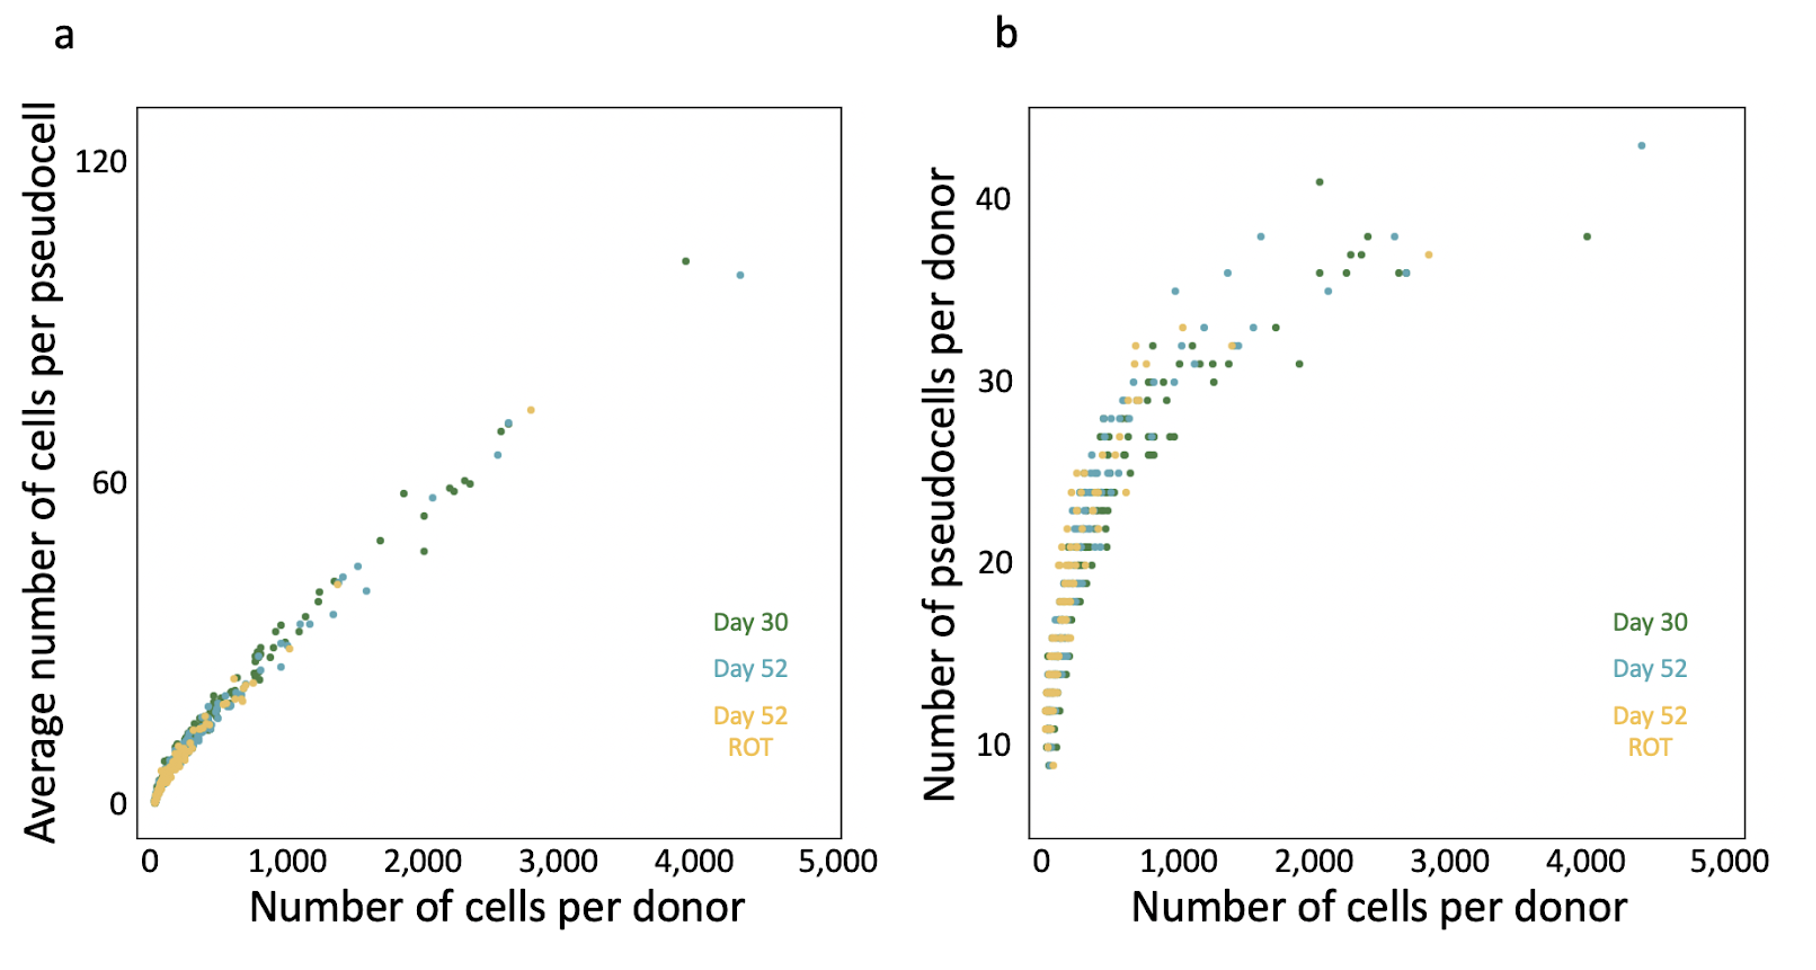
\includegraphics[width=13cm]{Appendix_CellRegMap/SuppFigures/Fig_S8.png}
    \caption{\textbf{Dopaminergic neuron pseudocell aggregation.}
    Transcriptionally related cells were aggregated into pseudocells, thereby reducing the sparsity in this dataset (dopaminergic neurons from \cite{jerber2021population}). 
    Pseudocells were constructed separately for each individual and conditions (day 30, day 52, rotenone-treated day 52; \textbf{Materials and Methods}).
    \textbf{(a)} Scatter plot between the number of cells for each individual (x axis) versus the average number of cells contained in a pseudocell for the corresponding individual (y axis). 
    Colour denotes the three main cell populations (collected across three conditions). 
    \textbf{(b)} Analogous as in a, comparing the number of cells per donor versus the number of pseudocells per donor.
}
\end{figure}


\begin{figure}[h]
    \centering
    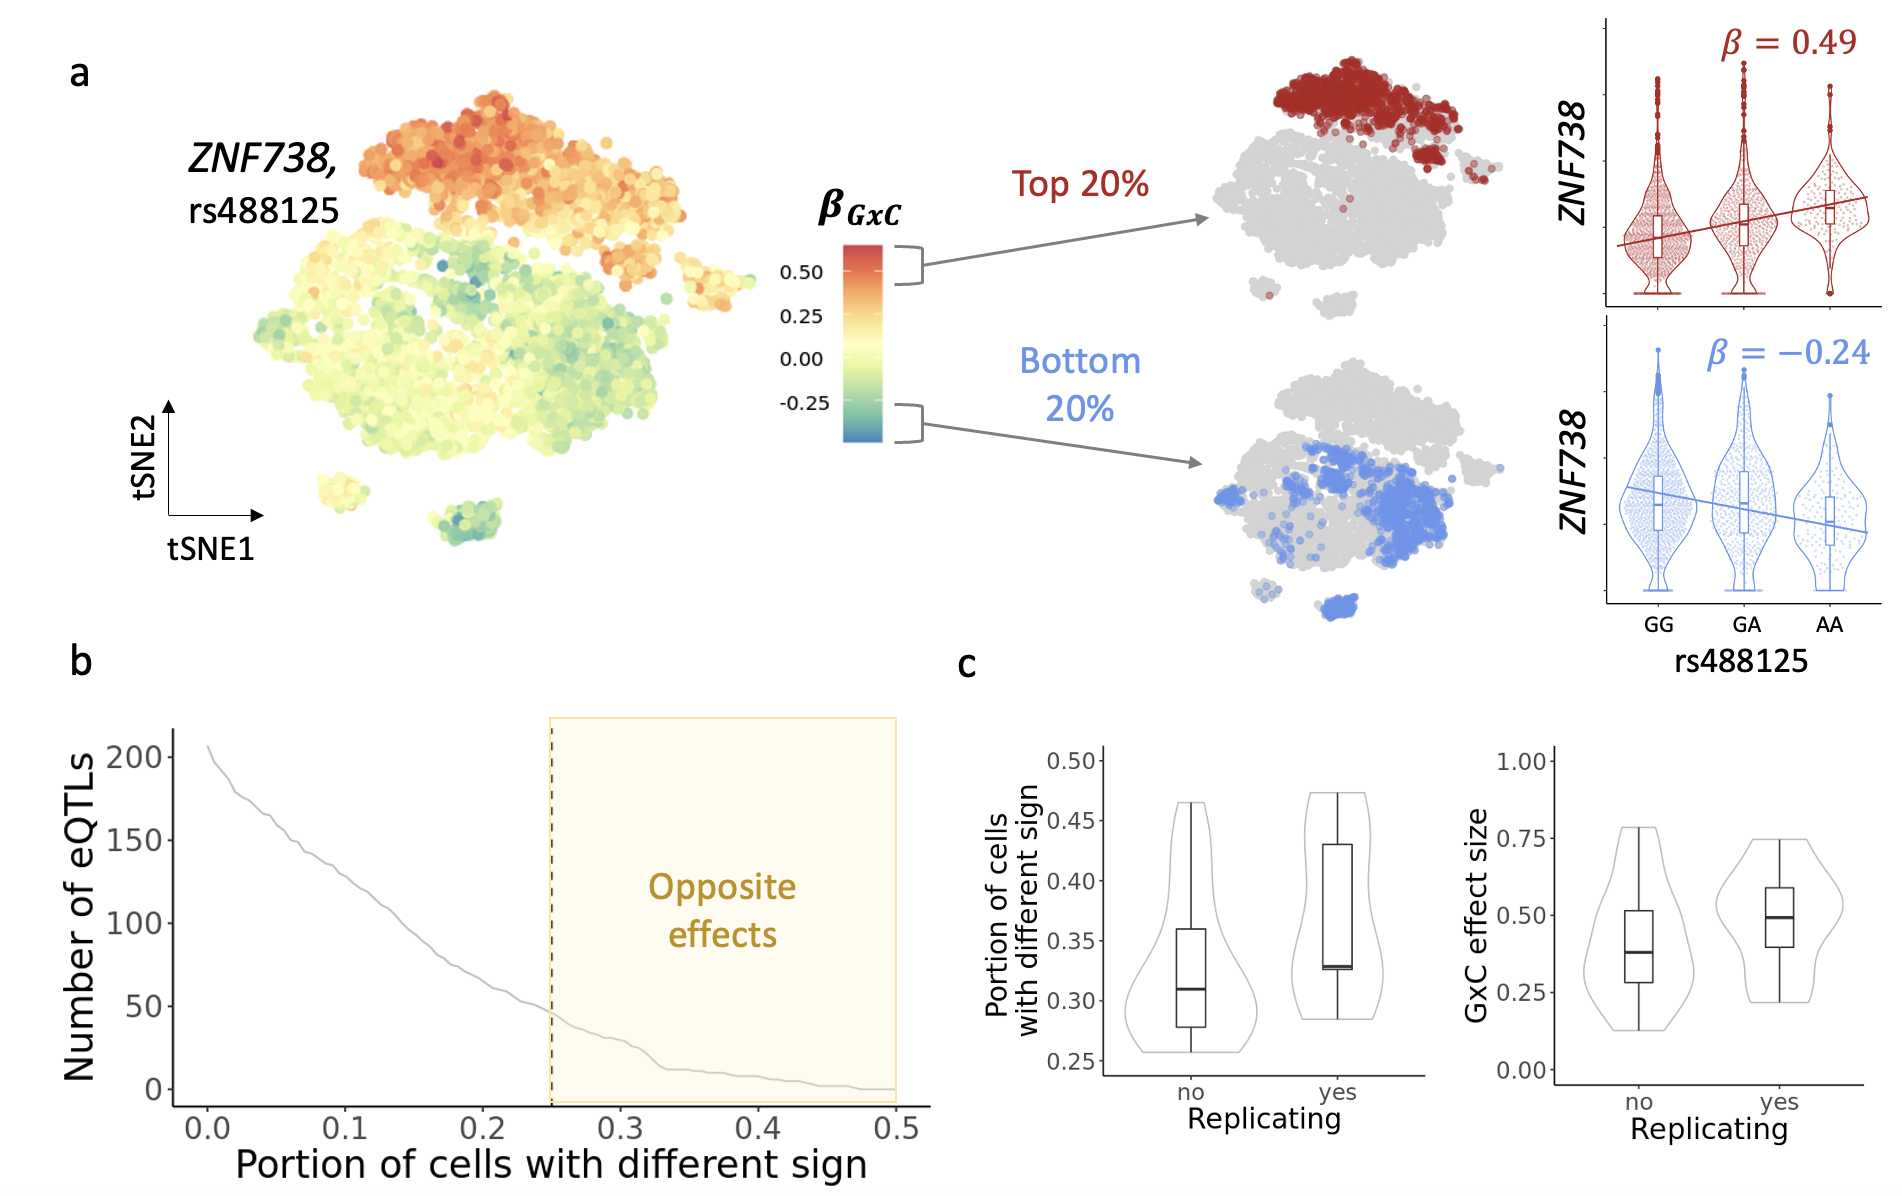
\includegraphics[width=16cm]{Appendix_CellRegMap/SuppFigures/Fig_S9.png}
    \caption{\textbf{Opposite effects detected by GxC.} 
    Considering data from \cite{cuomo2020single}. 
    \textbf{(a)} Example of “true” opposite effects. 
    The estimated genetic effects due to GxC (GxC) across all cells for the depicted eQTL (gene: \textit{ZNF738}, SNP: chr19:21474173) indicates opposite effects across different populations, as shown by the tSNE plot on the left. 
    To further assess this effect, we considered two extreme strata of cells (top and bottom 20\% of the GxC values, tSNE plots in the middle) and assessed direction of effect in each stratum using a standard eQTL mapping strategy (based on pseudo bulk mapping; \textbf{Materials and Methods}), demonstrating true opposite effects (box plots on the right). 
    \textbf{(b)} Distribution of the portion of cells with different sign from the rest in the GxC values (0 corresponds to the setting that indicates that GxC estimates for a given eQTL variant have consistent sign across all cells; 0.5 corresponds to 50\% of all cells having an opposite effect signtake on assumes only positive values across all cells only, 1 negative for all cells), for all significant GxC eQTL (n=213, FDR$<$5\%; neuronal development data). 
    We define a GxC eQTL as displaying opposite effects when at least 25\% of cells have a different sign compared to the rest in the estimated GxC values.
    \textbf{(c)} Next, we considered the 45 opposite effects from \textbf{(b)}, and assessed replication, by mapping standard eQTL when considering the top and bottom 20\% of cells (based on GxC values, as shown for the example in a). 
    When comparing the opposite effects that do replicate (opposite effect sizes using standard strategies as described in a; \textbf{Materials and Methods}) to those that do not replicate, we observe that (left) portion of cells with different signs is higher for the replicating ones (closer to a 50-50 split between positive and negative values), and (right) the estimated magnitude of GxC effect sizes (calculated as the delta of the top and bottom 10\% of GxC values) is lower for the non-replicating opposite effects.
}
\end{figure}

\begin{figure}[h]
    \centering
    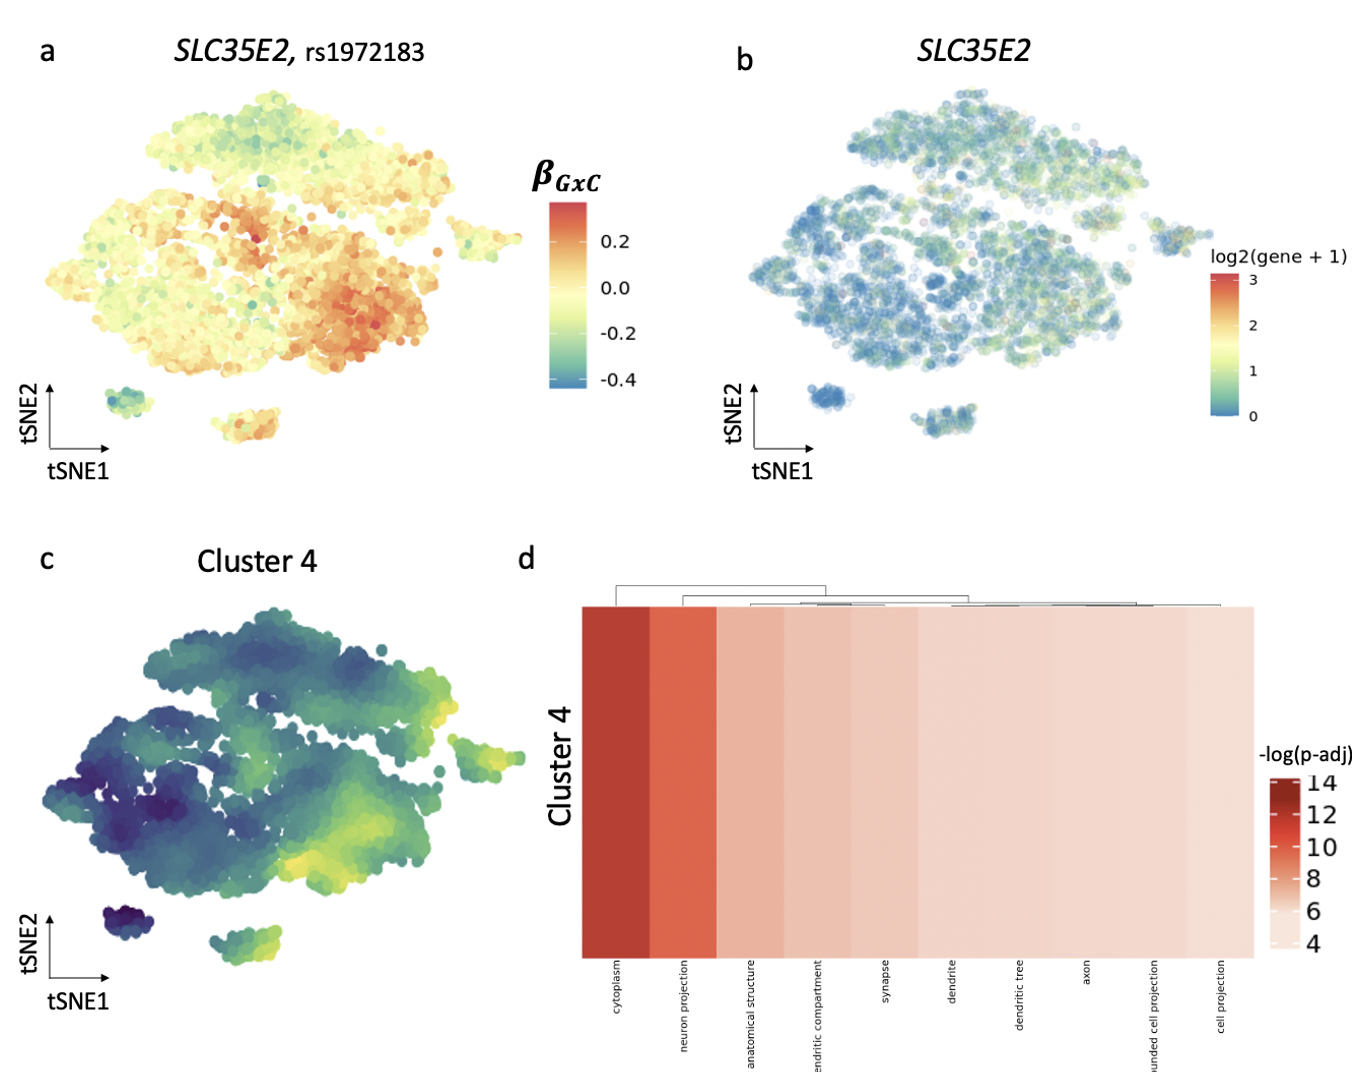
\includegraphics[width=14cm]{Appendix_CellRegMap/SuppFigures/Fig_S10.png}
    \caption{\textbf{CellRegMap to fine-map cellular context for human disease variant.} 
    Considering the subset of cells identified as dopaminergic neurons from \cite{jerber2021population}. \textbf{(a)} GxC profile at rs1972183 for \textit{SLC35E2}, which is colocalized with a GWAS variant for sleeplessness and insomnia in the subpopulation of day 52 untreated cells. 
    Shown is a scatter plot of the first two tSNE coordinates with colour denoting the estimated GxC effect component GxC. 
    \textbf{(b)} As in \textbf{a}, with colour denoting \textit{SLC35E2} single-cell gene expression levels. 
    \textbf{(c)} Manifold of consensus relative GxC effect sizes estimates for cluster 4, which contains the GxC effects for \textit{SLC35E2}.  
    \textbf{(d)} Extract of the gene enrichment analysis for cluster 4 (based on \textbf{Fig. EV4b}).
}
\end{figure}

\begin{figure}[h]
    \centering
    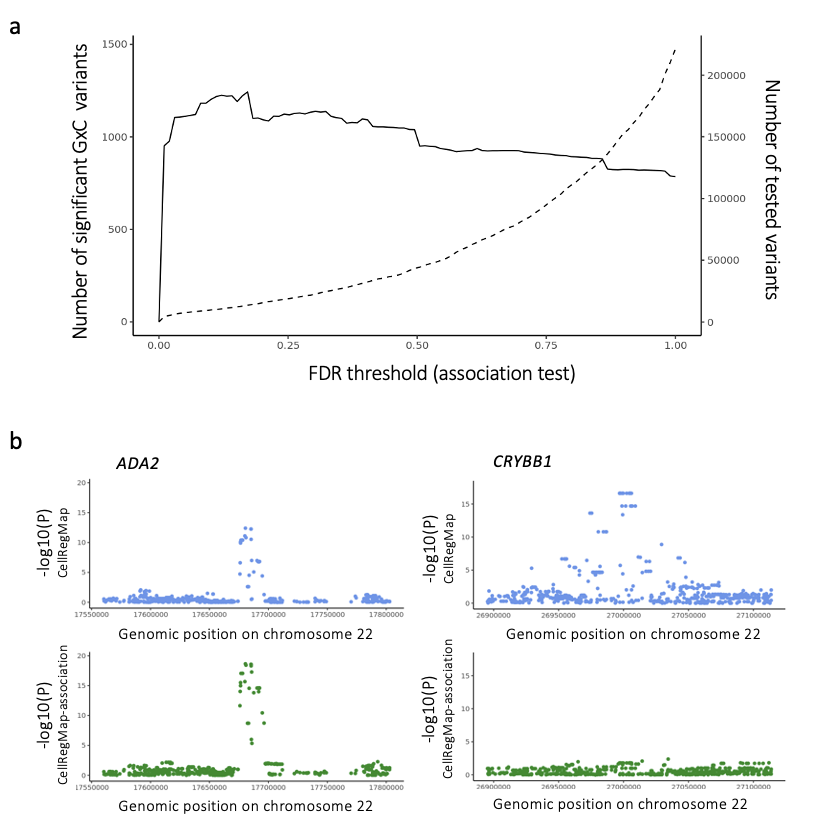
\includegraphics[width=13cm]{Appendix_CellRegMap/SuppFigures/Fig_S11.png}
    \caption{\textbf{Assessment of two-stage workflow using the CellRegMap-association test to define candidate eQTL for GxC analysis.} 
    Results based on the endoderm differentiation data \cite{cuomo2020single}, using the de-novo for both persistent effects using  the CellRegMap-association test and GxC interactions using the CellRegMap interaction test (+/- 100kb around the gene body, MAF$>$5\%, all expressed genes on chromosomes 20-22). 
    \textbf{(a)} Number of significant GxC effects (FDR$<$1\%; y-axis) as a function of the FDR threshold to filter for variants based on the association signal (x axis). 
    Second y-axis denotes the number of tested SNP-gene pairs. 
    While the number of tested SNP-gene pairs increases for less stringent filtering, the number of detected GxC effects decreases, indicating that no discoveries are lost when considering the top eQTL only, while computation time is saved, and power to find GxC is also (slightly) increased. 
    \textbf{(b)} Manhattan plots representing examples of same (left, for the \textit{ADA2} gene) vs different (right, for the \textit{CRYBB1} gene) signals being picked up by CellRegMap’s GxC interaction test (blue) and CellRegMap association test (green).
}
\end{figure}